\documentclass[hidelinks,12pt]{article}
\usepackage[left=0.25cm,top=1cm,right=0.25cm,bottom=1cm]{geometry}
%\usepackage[landscape]{geometry}
\textwidth = 20cm
\hoffset = -1cm
\usepackage[utf8]{inputenc}
\usepackage[spanish,es-tabla]{babel}
\usepackage[autostyle,spanish=mexican]{csquotes}
\usepackage[tbtags]{amsmath}
\usepackage{nccmath}
\usepackage{amsthm}
\usepackage{amssymb}
\usepackage{mathrsfs}
\usepackage{graphicx}
\usepackage{subfig}
\usepackage{standalone}
\usepackage[outdir=./Imagenes/]{epstopdf}
\usepackage{siunitx}
\usepackage{physics}
\usepackage{color}
\usepackage{float}
\usepackage{hyperref}
\usepackage{multicol}
%\usepackage{milista}
\usepackage{anyfontsize}
\usepackage{anysize}
%\usepackage{enumerate}
\usepackage[shortlabels]{enumitem}
\usepackage{capt-of}
\usepackage{bm}
\usepackage{relsize}
\usepackage{placeins}
\usepackage{empheq}
\usepackage{cancel}
\usepackage{wrapfig}
\usepackage[flushleft]{threeparttable}
\usepackage{makecell}
\usepackage{fancyhdr}
\usepackage{tikz}
\usepackage{bigints}
\usepackage{scalerel}
\usepackage{pgfplots}
\usepackage{pdflscape}
\pgfplotsset{compat=1.16}
\spanishdecimal{.}
\renewcommand{\baselinestretch}{1.5} 
\renewcommand\labelenumii{\theenumi.{\arabic{enumii}})}
\newcommand{\ptilde}[1]{\ensuremath{{#1}^{\prime}}}
\newcommand{\stilde}[1]{\ensuremath{{#1}^{\prime \prime}}}
\newcommand{\ttilde}[1]{\ensuremath{{#1}^{\prime \prime \prime}}}
\newcommand{\ntilde}[2]{\ensuremath{{#1}^{(#2)}}}

\newtheorem{defi}{{\it Definición}}[section]
\newtheorem{teo}{{\it Teorema}}[section]
\newtheorem{ejemplo}{{\it Ejemplo}}[section]
\newtheorem{propiedad}{{\it Propiedad}}[section]
\newtheorem{lema}{{\it Lema}}[section]
\newtheorem{cor}{Corolario}
\newtheorem{ejer}{Ejercicio}[section]

\newlist{milista}{enumerate}{2}
\setlist[milista,1]{label=\arabic*)}
\setlist[milista,2]{label=\arabic{milistai}.\arabic*)}
\newlength{\depthofsumsign}
\setlength{\depthofsumsign}{\depthof{$\sum$}}
\newcommand{\nsum}[1][1.4]{% only for \displaystyle
    \mathop{%
        \raisebox
            {-#1\depthofsumsign+1\depthofsumsign}
            {\scalebox
                {#1}
                {$\displaystyle\sum$}%
            }
    }
}
\def\scaleint#1{\vcenter{\hbox{\scaleto[3ex]{\displaystyle\int}{#1}}}}
\def\bs{\mkern-12mu}


\title{Polinomios asociados de Legendre \\[0.3em]  \large{Matemáticas Avanzadas de la Física}\vspace{-3ex}}
\author{M. en C. Gustavo Contreras Mayén}
%date{\today}
\begin{document}
\vspace{-4cm}
\maketitle
\fontsize{14}{14}\selectfont

%Ref. Butkov (1973) 9.8 Spherical Bessel Functions
\section{Polinomios asociados de Legendre.}

La principal utilidad de los polinomios asociados de Legendre es en la expansión de funciones definidas en la superficie de una esfera. Veamos el caso con la función de onda.
\par
Para cada frecuencia fija\footnote{Puede ser una eigenfrecuencia determinada a partir de la ecuación radial.} $\omega = k \, c$ le corresponde un modo:
\begin{align*}
\psi_{k} (\vb{r}, t) = \psi_{k} (\vb{r}) \, \exp(- i \omega t)
\end{align*}
donde $\psi_{k} (\vb{r})$ satisface la ecuación de Helmholtz:
\begin{align*}
\laplacian{\psi_{k}} + k^{2} \, \psi_{k} = 0
\end{align*}
Para resolver la ecuación, propongamos una separación de variables del tipo:
\begin{align*}
\psi_{k} (r, \theta, \phi) = R (r) \, Y (\theta, \phi)
\end{align*}
que nos lleva a:
\begin{align*}
\dv{r} \bigg( r^{2} \, \dv{R}{r} \bigg) &+ \big( k^{2} \, r^{2} + \lambda \big) \, R = 0 \\[0.5em]
\dfrac{1}{\sin \theta} \, \pdv{\theta} \bigg( \sin \theta \, \pdv{Y}{\theta} \bigg) &+ \dfrac{1}{\sin^{2} \theta} \, \pdv[2]{Y}{\phi} + \lambda \, Y = 0
\end{align*}
El eigenvalor $\lambda$ se determinará a partir de la segunda ecuación, tomemos en cuenta de que $Y (\theta, \phi)$ debe de ser finito para $0 \leq \theta \leq \pi$ y $0 \leq \phi \leq 2 \pi$, y tendremos eigenfunciones $Y_{\lambda} (\theta, \phi)$ correspondientes a esos eigenvalores.
\par
Entonces, la función completa $\phi_{k} (\vb{r})$ se puede expresar por una superposición del tipo:
\begin{align*}
\phi_{k} (\vb{r}) = \nsum_{\lambda} C_{\lambda} \, R_{\lambda} (r) \, Y_{\lambda} (\theta, \phi)
\end{align*}
\textbf{Nota: } La suma sobre $\lambda$ debe de considerarse como simbólica, ya que aún no hemos explorado la estructura del espectro de $\lambda$: ya sea continuo o discreto, ya sea que tenga o no degeneración.
\par
Para establecer los valores permitidos de $\lambda$, completamos la separación de variables, haciendo:
\begin{align*}
Y (\theta, \phi) = \Theta (\theta) \, \Phi (\phi)
\end{align*}
Lo que nos lleva a las ecuaciones:
\begin{align*}
\dv{\theta} \bigg( \sin \theta \, \dv{\Theta}{\theta} \bigg) + \bigg( - \sin \theta \lambda + \dfrac{\lambda_{1}}{\sin \theta} \bigg) \, \Theta &= 0 \\[0.5em]
\dv[2]{\Phi}{\phi} - \lambda_{1} \, \Phi &= 0
\end{align*}
las cuales ya hemos resuelto anteriormente. Sabemos que el espectro de $\lambda_{1}$ es discreto, sea $\lambda_{1}  - m^{2} ~ (m = 0, 1, 2, \ldots)$ y las eigenfunciones pueden definirse de la siguiente manera.
\par
\noindent
Para $m = 0$:
\begin{align*}
\Phi_{o} (\phi) = 1
\end{align*}
para $m \neq 0$:
\begin{align*}
\Phi_{m} (\phi) = \begin{cases}
\cos m \phi & \mbox{o bien} \\
\sin m \phi
\end{cases}
\end{align*}
Estas funciones son ortogonales entre sí y las integrales de normalización son:
\begin{align*}
\scaleint{6ex}_{\bs 0}^{2 \pi} \big[ \Phi_{0} (\phi) \big]^{2} \dd{\phi} &= 2 \, \pi \\[0.5em]
\scaleint{6ex}_{\bs 0}^{2 \pi} \cos^{2} m \, \phi \dd{\phi} &= \pi \\[0.5em]
\scaleint{6ex}_{\bs 0}^{2 \pi} \sin^{2} m \, \phi \dd{\phi} &= \pi
\end{align*}
Es conveniente en este momento tener esas eigenfunciones \emph{normalizadas a la unidad}, para ello las multiplicamos por las constantes apropiadas para que todas las integrales de normalización sean iguales a la unidad. Esta condición define las funciones normalizadas:
\begin{align*}
&\Phi_{0} (\phi) = \dfrac{1}{\sqrt{2 \pi}} \hspace{0.3cm} (m = 0) \\[0.5em]
&\left. \begin{aligned}
\Phi_{m}^{(+)} (\phi) &= \dfrac{1}{\sqrt{\pi}} \, \cos m \, \phi \\[0.5em]
\Phi_{m}^{(-)} (\phi) &= \dfrac{1}{\sqrt{\pi}} \, \sin m \, \phi
\end{aligned} \right\}
(m \neq 0)
\end{align*}
donde el símbolo $(+)$ o $(-)$ nos recuerda que esas funciones son pares o impares con respecto al intercambio $\phi \leftrightarrow - \phi$. En cuanto a las funciones $\Theta$ se refiere, sabemos que el espectro de $\lambda$ es también discreto, con:
\begin{align*}
\lambda = - \ell (\ell + 1) \hspace{0.5cm} \ell = 0, 1, 2, \ldots
\end{align*}
pero para cualquier $m$ dado, se tiene que $\ell \geq m$.
\par
Las soluciones de la ecuación con $\Theta$ son los polinomios asociados de Legendre $P_{\ell}^{m} (\cos \theta)$. Es conveniente normalizarlos a la unidad también, definiendo entonces:
\begin{align*}
\Theta_{\ell}^{m} (\cos \theta) = \sqrt{\dfrac{2 \ell + 1}{2} \, \dfrac{(\ell - m)!}{(\ell + m)!}} \, P_{\ell}^{m} (\cos \theta)
\end{align*}
por lo que:
\begin{align*}
\scaleint{6ex}_{\bs 0}^{\pi} \big[ \Theta_{\ell}^{m} (\cos \theta) \big]^{2} \sin \theta \dd{\theta} = \dfrac{2 \ell + 1}{2} \, \dfrac{(\ell - m)!}{(\ell + m)!} \, \scaleint{6ex}_{\bs -1}^{+1} \big[ P_{\ell}^{m}  (x) \big]^{2} \dd{x} = 1
\end{align*}

Ahora debería de quedar claro que la ecuación de eigenvalores:
\begin{align*}
\dfrac{1}{\sin \theta} \, \pdv{\theta} \bigg( \sin \theta \, \pdv{Y}{\theta} \bigg) &+ \dfrac{1}{\sin^{2} \theta} \, \pdv[2]{Y}{\phi} + \lambda \, Y = 0
\end{align*}
tiene los eigenvalores:
\begin{align*}
\lambda = - \ell (\ell + 1) \hspace{0.4cm} \ell = 0, 1, 2, \ldots
\end{align*}
que son, sin embargo, \emph{degenerados} (excepto si $\ell = 0)$, por que para cada valor fijo de $\ell$, se tiene varias eigenfunciones:
\begin{align*}
&\Theta_{\ell}^{0} (\cos \theta) \, \Phi_{0} (\phi) \\[0.5em]
&\Theta_{\ell}^{1} (\cos \theta) \, \Phi_{1}^{(+)} (\phi) \hspace{0.7cm} \Theta_{\ell}^{1} (\cos \theta) \, \Phi_{1}^{(-)} (\phi) \\[0.5em]
&\Theta_{\ell}^{2} (\cos \theta) \, \Phi_{2}^{(+)} (\phi) \hspace{0.7cm} \Theta_{\ell}^{2} (\cos \theta) \, \Phi_{2}^{(-)} (\phi) \\[0.5em]
&{} \hspace{0.3cm} \vdots
\end{align*}
y así sucesivamente, hasta llegar a:
\begin{align*}
\Theta_{\ell}^{\ell} (\cos \theta) \, \Phi_{2}^{(+)} (\phi) \hspace{0.5cm} \Theta_{\ell}^{\ell} (\cos \theta) \, \Phi_{2}^{(-)} (\phi)
\end{align*}
Para cada valor de $\ell$ le corresponden $(2 \ell + 1)$ eigenfunciones, teniendo entonces un orden de degeneración de $(2 \ell + 1)$.
\par
Definimos las soluciones fundamentales de la EDP (sujeta a las CDF apropiadas)
\begin{align*}
\dfrac{1}{\sin \theta} \, \pdv{\theta} \bigg( \sin \theta \, \pdv{Y}{\theta} \bigg) &+ \dfrac{1}{\sin^{2} \theta} \, \pdv[2]{Y}{\phi} + \ell (\ell + 1) \, Y = 0
\end{align*}
por medio de las expresiones:
\begin{align*}
&Y_{\ell 0} (\theta, \phi) = \sqrt{\dfrac{2 \ell + 1}{4 \pi}} \, P_{\ell} (\cos \theta) \hspace{0.3cm} (m = 0) \\[0.5em]
&\left. \begin{aligned}
Y_{\ell m}^{(+)} (\theta, \phi)  (\phi) &= \Theta_{\ell}^{m} (\cos \theta) \, \Phi_{m}^{(+)} (\phi) = \\[0.5em]
&= \sqrt{\dfrac{2 \ell + 1}{2 \pi} \, \dfrac{(\ell - m)!}{(\ell + m)!}} \, P_{\ell}^{m} (\cos \theta) \, \cos m \phi \\[0.5em]
Y_{\ell m}^{(-)} (\theta, \phi)  (\phi) &= \Theta_{\ell}^{m} (\cos \theta) \, \Phi_{m}^{(-)} (\phi) = \\[0.5em]
&= \sqrt{\dfrac{2 \ell + 1}{2 \pi} \, \dfrac{(\ell - m)!}{(\ell + m)!}} \, P_{\ell}^{m} (\cos \theta) \, \sin m \phi
\end{aligned} \right\}
(m \neq 0)
\end{align*}
Estas soluciones son los armónicos esféricos (en la definición clásica\footnote{De manera contraria en la definición de los armónicos esféricos en la mecánica cuántica, donde $\cos m \phi$ y $\sin m \phi$ se descartan en favor de $\exp(i m \phi)$ y $\exp(-i m \phi)$.}).
\par
Se sigue entonces que la expresión en series para $\psi_{k} (\vb{r})$ es del tipo:
\begin{align*}
\psi_{k} (\vb{r}) = \nsum_{\lambda} C_{\lambda} \, R_{\lambda} (r) \, Y_{\lambda} (\theta, \phi)
\end{align*}
que es de la forma:
\begin{align*}
\psi_{k} (\vb{r}) = \nsum_{\ell=0}^{\infty} R_{\ell} (r) \bigg[ C_{\ell 0} \, Y_{\ell 0} (\theta, \phi) {+} \nsum_{m=1}^{\ell} \bigg( C_{\ell m}^{(+)} \, Y_{\ell m}^{(+)} (\theta, \phi) + C_{\ell m}^{(-)} \, Y_{\ell m}^{(-)} (\theta, \phi) \bigg) \bigg]
\end{align*}

Supongamos que $r$ está fijo, entonces $\psi_{k} (\vb{r})$ se convierte en una función solo de $\theta$ y $\phi$, por lo que estaremos tratando con una expresión del tipo:
\begin{align*}
f (\theta, \phi) = \nsum_{\ell=0}^{\infty} \bigg[ A_{\ell 0} \, Y_{\ell 0} (\theta, \phi) {+} \nsum_{m=1}^{\ell} \bigg( A_{\ell m}^{(+)} \, Y_{\ell m}^{(+)} (\theta, \phi) + A_{\ell m}^{(-)} \, Y_{\ell m}^{(-)} (\theta, \phi) \bigg) \bigg]
\end{align*}
Esta expansión en serie es válida para una función arbitraria $f (\theta, \phi)$, sujeta a las condiciones habituales similares para las series de Fourier, series de Fourier-Legendre, series de Fourier-Bessel, etc.
\par
Los coeficientes de la expansión se obtienen multiplicando $f (\theta, \phi)$ por el correspondiente armónico esférico y por el factor $\sin \theta$, para luego integrar sobre los ángulos:
\begin{align*}
A_{\ell 0} &= \scaleint{6ex}_{\bs 0}^{\pi} \scaleint{6ex}_{\bs 0}^{2 \pi} f (\theta, \phi) \, Y_{\ell 0} (\theta, \phi) \, \sin \theta \dd{\theta} \hspace{0.5cm} (m = 0) \\[0.5em] 
A_{\ell m}^{(\pm)} &= \scaleint{6ex}_{\bs 0}^{\pi} \scaleint{6ex}_{\bs 0}^{2 \pi} f (\theta, \phi) \, Y_{\ell 0}^{(\pm)} (\theta, \phi) \, \sin \theta \dd{\theta} \hspace{0.5cm} (m \neq 0)
\end{align*}

\emph{Observación: } El factor $\sin \theta$ que se necesita para la ortogonalidad de las funciones $P_{\ell}^{m}$, tiene la siguiente interpretación geométrica: Un ángulo sólido se define por:
\begin{align*}
\dd{\Omega} = \dfrac{\dd{S}}{r^{2}}
\end{align*}
donde $\dd{S}$ es el elemento de área de una esfera de radio $r$. En el sistema esférico:
\begin{align*}
\dd{S} = r \, \dd{\theta} \, r \, \sin \theta \dd{\phi}
\end{align*}
tal que:
\begin{align*}
\dd{\Omega} = \sin \theta \dd{\theta} \dd{\phi}
\end{align*}
y las integrales citadas anteriormente pueden considerarse integrales sobre el ángulo sólido y escribirse simbólicamente como:
\begin{align*}
A_{\ell 0} = \scaleint{6ex}_{\Omega} f (\Omega) \, Y_{\ell 0} (\Omega) \dd{\Omega} \hspace{0.5cm} (m = 0) \\[0.5em]
A_{\ell m}^{\pm} = \scaleint{6ex}_{\Omega} f (\Omega) \, Y_{\ell m}^{\pm} (\Omega) \dd{\Omega} \hspace{0.5cm} (m \neq 0)
\end{align*}

\section{Las funciones esféricas de Bessel.}

Continuemos revisando las EDP de onda y de Helmholtz en coordenadas esféricas. Sabemos que la ecuación radial es de la forma:
\begin{align*}
\dv{r} \bigg( r^{2} \, \dv{R}{r} \bigg) + \big[ k^{2} \, r^{2} - \ell (\ell + 1) \big] \, R = 0 \hspace{0.5cm} \ell = 0, 1, 2, \ldots
\end{align*}
Si hacemos el cambio de variable $x = k \, r$ $y (x) \equiv R (r)$, la ecuación se reduce a:
\begin{align*}
x^{2} \, \dv[2]{y}{x} + 2 \, x \, \dv{y}{x} + \big[ x^{2} - \ell (\ell + 1) \big] \, y = 0
\end{align*}
Las soluciones de esta ED se conocen como las \emph{funciones esféricas de Bessel} y las funciones \emph{esféricas de Neumann} de orden $\ell$, escritas como $j_{\ell} (x)$ y $n_{j} (x)$, respectivamente.
\par
La razón de darles ese nombre es debido al cambio de variable:
\begin{align*}
y (x) = \dfrac{u (x)}{\sqrt{x}}
\end{align*}
reduce la ecuación a la forma:
\begin{align*}
\dv[2]{u}{x} + \dfrac{1}{x} \dv{u}{x} + \bigg[ 1 - \dfrac{\big( \ell + \frac{1}{2} \big)}{x^{2}} \bigg] \, u = 0 \hspace{0.5cm} \ell = 0, 1, 2, \ldots
\end{align*}
que reconocemos es la ED de Bessel de orden $\ell + 1/2$. Se sigue entonces que las soluciones de la ED inicial, pueden escribirse de la forma:
\begin{align*}
y (x) = C_{1} \, \dfrac{J_{\ell+1/2} (x)}{\sqrt{x}} + C_{2} \, \dfrac{J_{-\ell-1/2} (x)}{\sqrt{x}}
\end{align*}
y si la función de Bessel esférica $j_{\ell} (x)$ se define como una solución finita en $x = 0$, se sigue que debe ser un múltiplo de $J_{\ell+1/2} (x) / \sqrt{x}$. El factor de proporcionalidad generalmente se elige para que sea $\sqrt{\pi/2}$, por lo tanto:
\begin{align*}
j_{\ell} (x) = \sqrt{\dfrac{\pi}{2 x}} \, J_{\ell+1/2} (x)
\end{align*}
La relación de las $j_{\ell} (x)$ con las funciones de Bessel, nos permiten expresar las $j_{\ell} (x)$ en términos de $j_{0} (x)$. De la expresión:
\begin{align*}
J_{\mu+1} (x) = - x^{\mu} \, \dv{x} \bigg[ \dfrac{J_{\mu} (x)}{x^{\mu}} \bigg]
\end{align*}
que entonces, al hacer $\mu = \ell + 1/2$ y dividiendo entre $x^{\ell+3/2}$, se tiene:
\begin{align*}
\dfrac{J_{\ell+3/2} (x)}{x^{\ell+3/2}} &= - \dfrac{1}{x} \, \dv{x} \bigg[ \dfrac{J_{\ell+1/2} (x)}{x^{\ell+1/2}} \bigg] \\[0.5em]
\mbox{o } \hspace{0.3cm} \dfrac{j_{\ell+1} (x)}{x^{\ell+1}} &= - \dfrac{1}{x} \dv{x} \bigg[ \dfrac{j_{\ell} (x)}{x^{\ell}} \bigg]
\end{align*}
Comenzando con $\ell = 0$ y ocupando esta expresión $\ell$ veces, se obtiene:
\begin{align*}
j_{\ell} (x) = x^{\ell} \bigg( - \dfrac{1}{x} \, \dv{x} \bigg)^{\ell} \, j_{0} (x) \hspace{0.5cm} \ell = 1, 2, \ldots 
\end{align*}
Esta expresión únicamente define todas las $j$ funciones una vez que $j_{0}$ se elige. Nuestra ecuación para $\ell = 0$ es entonces:
\begin{align*}
\dv[2]{y}{x} + \dfrac{2}{x} \, \dv{y}{x} + y = 0
\end{align*}
Resolviendo esta ecuación (ya sea por Frobenius o por otro método), encontramos que las funciones $\sin x /x$ y $\cos x /x$ están entre las soluciones. Es común definir:
\begin{align*}
j_{0} (x) = \dfrac{\sin x}{x}
\end{align*}
en comparación con $J_{1/2}$, se tiene:
\begin{align*}
j_{0} (x) = \sqrt{\dfrac{\pi}{2 x}} \, J_{1/2} (x)
\end{align*}
que explica el factor $\sqrt{\pi / 2}$.
\par
Las funciones esféricas de Neumann $n_{\ell} (x)$ se generan de manera similar a partir de $n_{0} (x)$ por medio de:
\begin{align*}
n_{\ell} (x) = x^{\ell} \bigg( - \dfrac{1}{x} \, \dv{x} \bigg)^{\ell} \, n_{0} (x) \hspace{0.5cm} \ell = 1, 2, \ldots
\end{align*}
siendo común definir:
\begin{align*}
n_{0} (x) = - \dfrac{\cos x}{x} = \sqrt{\dfrac{\pi}{2 x}} \, J_{-1/2} (x)
\end{align*}

A continuación se presenta una lista con algunas funciones $j_{\ell} (x)$:
\begin{align*}
j_{0} (x) &= \dfrac{\sin x}{x} \\[0.5em]
j_{1} (x) &= \dfrac{\sin x}{x^{2}} - \dfrac{\cos x}{x} \\[0.5em]
j_{2} (x) &= \bigg( \dfrac{3}{x^{3}} - \dfrac{1}{x} \bigg) \, \sin x - \dfrac{3}{x^{2}} \, \cos x \\[0.5em]
j_{3} (x) &= \bigg( \dfrac{15}{x^{4}} - \dfrac{6}{x^{2}} \bigg) \, \sin x - \bigg( \dfrac{15}{x^{3}} - \dfrac{1}{x} \bigg) \, \cos x 
\hspace{0.4cm} &\vdots
\end{align*}
\begin{figure}[H]
    \centering
    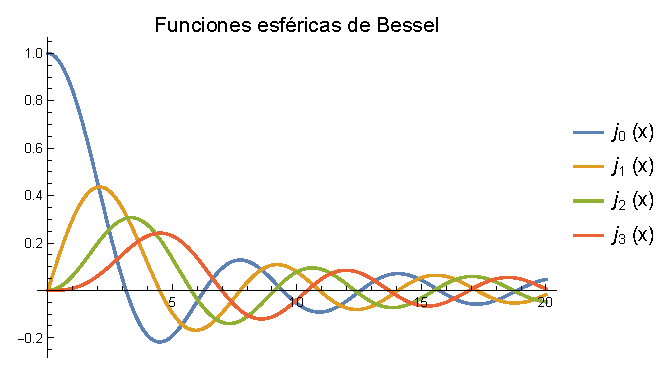
\includegraphics[scale=1]{Imagenes/Plot_Esfericas_Bessel.eps}
\end{figure}

En la siguiente lista ahora presentamos algunas funciones $n_{\ell} (x)$:
\begin{align*}
n_{0} (x) &= - \dfrac{\cos x}{x} \\[0.5em]
n_{1} (x) &= - \dfrac{\cos x}{x^{2}} - \dfrac{\sin x}{x} \\[0.5em]
n_{2} (x) &= - \bigg( \dfrac{3}{x^{2}} - \dfrac{1}{x} \bigg) \, \cos x - \dfrac{3}{x^{2}} \, \sin x \\[0.5em]
n_{3} (x) &= - \bigg( \dfrac{15}{x^{4}} - \dfrac{6}{x^{2}} \bigg) \, \cos x - \bigg( \dfrac{15}{x^{3}} - \dfrac{1}{x} \bigg) \, \sin x
\end{align*}
\begin{figure}[H]
    \centering
    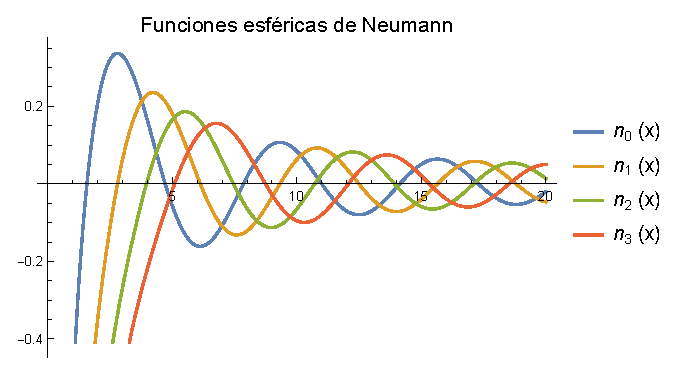
\includegraphics[scale=1]{Imagenes/Plot_Esfericas_Neumann.eps}
\end{figure}
\end{document}